
\documentclass{article}

% if you need to pass options to natbib, use, e.g.:
% \PassOptionsToPackage{numbers, compress}{natbib}
% before loading nips_2016
%
% to avoid loading the natbib package, add option nonatbib:
% \usepackage[nonatbib]{nips_2016}

%\PassOptionsToPackage{numbers, compress}{natbib}
\usepackage[final]{nips_2016}
\bibliographystyle{unsrt}
\usepackage[pdftex]{graphicx}
\bibliographystyle{prsty}


% to compile a camera-ready version, add the [final] option, e.g.:
% \usepackage[final]{nips_2016}

\usepackage[utf8]{inputenc} % allow utf-8 input
\usepackage[T1]{fontenc}    % use 8-bit T1 fonts
\usepackage{hyperref}       % hyperlinks
\usepackage{url}            % simple URL typesetting
\usepackage{booktabs}       % professional-quality tables
\usepackage{amsfonts}       % blackboard math symbols
\usepackage{nicefrac}       % compact symbols for 1/2, etc.
\usepackage{microtype}      % microtypography
\usepackage{caption}
\usepackage{todonotes}
%\usepackage{float}
\usepackage{subcaption}

\title{ChromaNet: Deep neural networks for chromatin profile prediction}

% The \author macro works with any number of authors. There are two
% commands used to separate the names and addresses of multiple
% authors: \And and \AND.
%
% Using \And between authors leaves it to LaTeX to determine where to
% break the lines. Using \AND forces a line break at that point. So,
% if LaTeX puts 3 of 4 authors names on the first line, and the last
% on the second line, try using \AND instead of \And before the third
% author name.

\author{ % add your first name and last name don't think we need to add dprt and emails for this project
  Adithya Ganesh \And Behrooz Ghorbani \And Philip Hwang \AND Wendi Liu  \And Armin Pourshafeie  \And Karen Yang
}

\begin{document}
% \nipsfinalcopy is no longer used

\maketitle

\begin{abstract}
In this work, we apply deep neural networks to the problem of {\it de novo} chromatin profile prediction.  Our analysis takes two broad approaches.  First, to model long-term dependencies, we train a purely recurrent neural network.  In particular, a bidirectional-LSTM network was used directly on the sequence, which outperformed a logistic regression baseline.  Secondly, we train a convolutional neural network adapted from the DeepSEA architecture \cite{zhou2015predicting}, to analyze the benefits of multitask learning. We use principal component analysis to identify clusters of tasks, and give evidence that training a network on related tasks improves PR-AUC performance relative to randomly selected tasks.

%Our analysis takes two broad approaches. 

%1) To take long-range correlations into consideration, we train a purely recurrent network. 2) We explore the benefits of multi-task learning in a DeepSEA like model to understand the marginal benefits of adding tasks and data as well as to identify clusters that may be informative when learned together.

% * <ghorbani@stanford.edu> 2016-11-17T19:01:23.366Z:
%
% This is very nice but usually it comes in the introduction rather than abstract
%
% ^.
% Understanding the functionality of non-coding genomic variants is of paramount importance, as the majority of disease-associated variants lie in these regions [Citation Needed / we can mention 93 percent].  Various research works have developed scoring methods, such as CADD [3] and PolyPhen [4], that aim to quantify the pathogenicity of a variant. These algorithms largely rely on population-dependent statistics, such as alternate allele frequencies.
\end{abstract}

\section{Introduction}
Understanding the functionality of non-coding genomic variants is of paramount importance, as approximately 93\% of disease associated variants are in non-coding regions \cite{maurano2012systematic}. Various methods have been developed to score the pathogenicity of particular variants.  One example is CADD \cite{kircher2014general}, which uses a support vector machine model to estimate pathogenicity based on various metrics that include chromatin structure, conservation metrics and transcription information. 
%(for examples see  CADD [3] PolyPhen [4]% I'm pretty sure polyphen is protein only%)

More recently, Zhou et al. \cite{zhou2015predicting} and Quang et al. \cite{quang2016danq} applied deep learning methods to predict chromatin profile {\it de novo}, using only sequence information. The predicted chromatin profile can then be used to model functional effects.  The DeepSEA model \cite{zhou2015predicting}  uses three convolutional layers which serve as spatial motif detectors. In their DanQ model, Quang et al. use a single convolutional layer followed by a bi-directional LSTM layer to model long-term interactions. Both methods are designed to predict the chromatin profile for a 200-bp sequence window with a 400-bp of additional context on each side.

Because both DeepSEA and DanQ employ convolutional layers, they require a fixed input length (1000-bp).  Zhou et al. \cite{zhou2015predicting} have demonstrated that training DeepSEA models with inputs of larger context size results in increased prediction accuracy (see Figure \ref{figs:context-acc}). This observation is consistent with the fact that spatially distant sites are known to exhibit co-dependent behavior.  For example, the ZRS regulator, which plays a role in modulating anatomical structure of tetrapod limbs, lies 1Mb from the target gene {\it Shh} \cite{lettice2003long}.  In this research, we demonstrate a proof-of-concept fully-recurrent network, which can be extended to model these very distant dependencies.

\begin{figure}[h]
\begin{center}
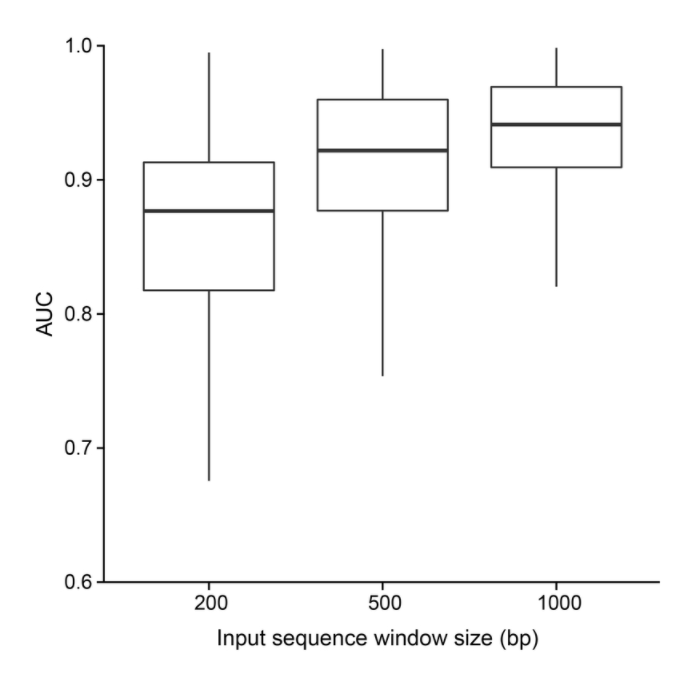
\includegraphics[width=.6\textwidth]{figures/context-acc.png}
\caption{Prediction accuracy with different context length}
\label{figs:context-acc}
\end{center}
\end{figure}

The networks in both DeepSEA and DanQ are trained in a joint multi-task fashion to simultaneously learn to predict transcription factor (TF) binding, DNase I-hypersensitive sites, and histone marks across multiple cell types. However, multitask learning does not always improve performance \cite{caruana1998multitask}.  We are interested in characterizing the performance of different multitask learning formulations, and in particular determining whether certain tasks are antagonistic to model performance.

To address the ideas above, we trained two different neural network models: a) a convolutional neural network, and b) a bidirectional-LSTM recurrent network.  Using the convolutional network, we find that perhaps unsurprisingly, increasing the number of tasks increasing the performance.  We also find preliminary evidence that suggests training similar tasks together improves test performance.  Specifically, training DNase tasks together resulted in better performance than training randomly selected tasks.

We also trained a bidirectional LSTM network that outperformed a logistic regression baseline.  This demonstrates an important proof of concept, as fully recurrent architectures are well suited to modeling long-term dependencies and variable-length inputs \cite{zhou2016deep} \cite{cho2014learning} \cite{kalchbrenner2013recurrent} \cite{sutskever2014sequence}.

\section{Related Work}

\subsection{Chromatin profile prediction}
Traditionally, analyzing genome sequences involves searching for common motifs or applying phylogenetic comparison.  This often requires prior knowledge of motifs, expert annotations, or applying motif discovery algorithms \cite{jaspar} \cite{wang2012sequence}.
 
Several recent studies have adopted weighted k-mer scoring or gapped k-mer scoring to train a discriminative model to discover potential new motifs from known motif databases \cite{ghandi2014enhanced} \cite{lee2016ls} \cite{choi2002analysis}.  These studies use a set of k-mer features on ChIP-seq / DNase-seq peaks (positive examples) versus their flanks (negative examples), to predict the activity of sequence elements, typically ranging from 500 to 2000 bp in length. To eliminate the limitations of short k-mer frequency features in representing longer TB binding sites, gapped k-mers features are shown to significantly improve sequence classification accuracy.\cite{ghandi2014enhanced}  Another approach that applies SVMs is the CADD algorithm \cite{kircher2014general}, where Kircher et.al introduced C-scores that correlate with a range of features, including allelic diversity, disease severity, and complex trait associations.

\subsection{Chromatin profile prediction with neural networks}

A number of research efforts have applied deep neural networks to predict chromatin profile from sequence.  While classical algorithms like support vector machines require manual preprocessing and feature selection, deep neural networks can adaptively extract features from the data during training \cite{kelley2016basset}.

Convolutional neural networks (CNNs) are one of the most successful deep learning architectures that have been applied to chromatin profile prediction, often out-performing classical methods such as gkm-svm \cite{kelley2016basset} \cite{zhou2015predicting} \cite{deepBind}. For instance, DeepBind \cite{deepBind} uses 16 convolutional layers with window size of 24, a global max-pooling layer, and a fully connected layer of size 32 with a dropout layer.  The DeepSEA model \cite{zhou2015predicting} uses a context sequence size of 1 kb, and uses a  hierarchical architecture of three convolution layers with 320, 480 and 960 kernels, and adopts multi-task joint learning of diverse chromatin factors sharing predictive features in the final sigmoid output layer.

By contrast, recurrent neural networks (RNNs) are comparatively less studied.  Bidirectional-RNNs \cite{BRNN} are capable of modeling interactions from future and past inputs. A variant of the BRNN model, the bidirectional Long Short-Term Memory (BLSTM) network, consists of gates which are added on each layer that control the degree of influence of information from the current step, and from the previous and next steps. This enables the model to capture the long-term temporal dependencies in sequential data with more control and flexibility.  Quang et al. \cite{quang2016danq} used a combination of CNNs and bidirectional LSTMs to capture time dependencies on features extracted by convolutional operations.

\subsection{Multi-task Learning}
Multi-task neural architectures provide a joint learning framework for simultaneous feature sharing across many different but related learning tasks. In this setting, the network parameters are shared, with only the last layers of the network being task specific. It is expected that sharing deep layers would improve features produced by these deep layers, and thus improve generalization performance, as well as compensating for the imbalanced data distributions for one single task. Many recent empirical studies have shown the benefits of multi-task learning. Ramsundar et al. \cite{ramsundar2015massively} found that multi-task networks can help in situations of imbalanced datasets that require special handling for effective learning. They found multi-task methods obtain predictive accuracies significantly better than single-task ones, and the presence of shared active compounds was correlated with multi-task improvement.  However, multitask learning does not always improve performance \cite{caruana1998multitask}, and thus it is often treated as a tool that requires testing on each application.

\section{Dataset and pre-processing}
Both of our frameworks use the same data used in the DanQ and DeepSEA models \cite{quang2016danq} \cite{zhou2015predicting}. To prepare this data, human reference genome (GRCH37) was segmented into non-overlapping 200bp windows. The binary labels for each task were determined by intersecting the windows with 919 ChIP-seq and DNase peaks determined by the ENCODE \cite{encode2012integrated} and Roadmap Epigenomics \cite{kundaje2015integrative} projects. Each region contains 400 flanking bases on each side for a total of 1000bp per region. Each window was one-hot encoded into a $1000 \times 4$ matrix. The dataset was augmented with the reverse complement of these regions.  Training, validation and test sets were designed to contain strictly non-overlapping chromosomes.  Due to computational limitations, we have sub-sampled the data as described in the corresponding section below.

\section{Architecture}
We performed experiments with a convolutional and recurrent neural network, which we discuss below.

\subsection{Convolutional Network}
In order to explore the performance characeristics of multi-task learning, we used a convolutional architecture similar to the DeepSEA model \cite{zhou2015predicting}. In particular, we use three convolutional layers with 320, 480 and 960 kernels from bottom to top.  Each kernel has a window of length 8 with max-pooling of window size 4, and the final prediction is made after a fully connected layer.  

While both \cite{zhou2015predicting,quang2016danq} used multi-task learning, the benefits of this approach for the problem of chromatin structure prediction has not been studied in detail. While the sheer number of proteins and cell-types requires a multi-task learning approach, the following problems are underexplored:
\begin{itemize}
\item The performance impact of adding tasks
\item The performance impact of adding data
\item The performance impact selecting tasks to be learned together
\end{itemize}
In this section of our project, we aim at investigating the performance impact of these choices.

We have used the data curated by DeepSEA \cite{zhou2015predicting}, where 200bp sequences with 400bp flanking context, and their reverse complements are one-hot encoded. Due to computational limitations we used the first 1M regions for training (out of the total of 4.4M training regions used in previous work \cite{zhou2015predicting,quang2016danq}) and 200k random regions for testing (more than 400k regions provided). However, we keep the validation set as in the aforementioned works (8,000 regions). 

\subsubsection{Experiments with weighted cost function}
Figure \ref{fig:frequency} shows the frequency of positive examples in our training data. Two facts are apparent from the figure:
\begin{enumerate}
\item Across all the tasks, the data is extremely unbalanced. 
\item The number of positive examples is highly dependent on the nature of the task. For example, TF binding factors have extremely low number of positive responses while histone marks can have up to $20\%$ positive examples. 
\end{enumerate}

\begin{figure}[h]
\begin{center}
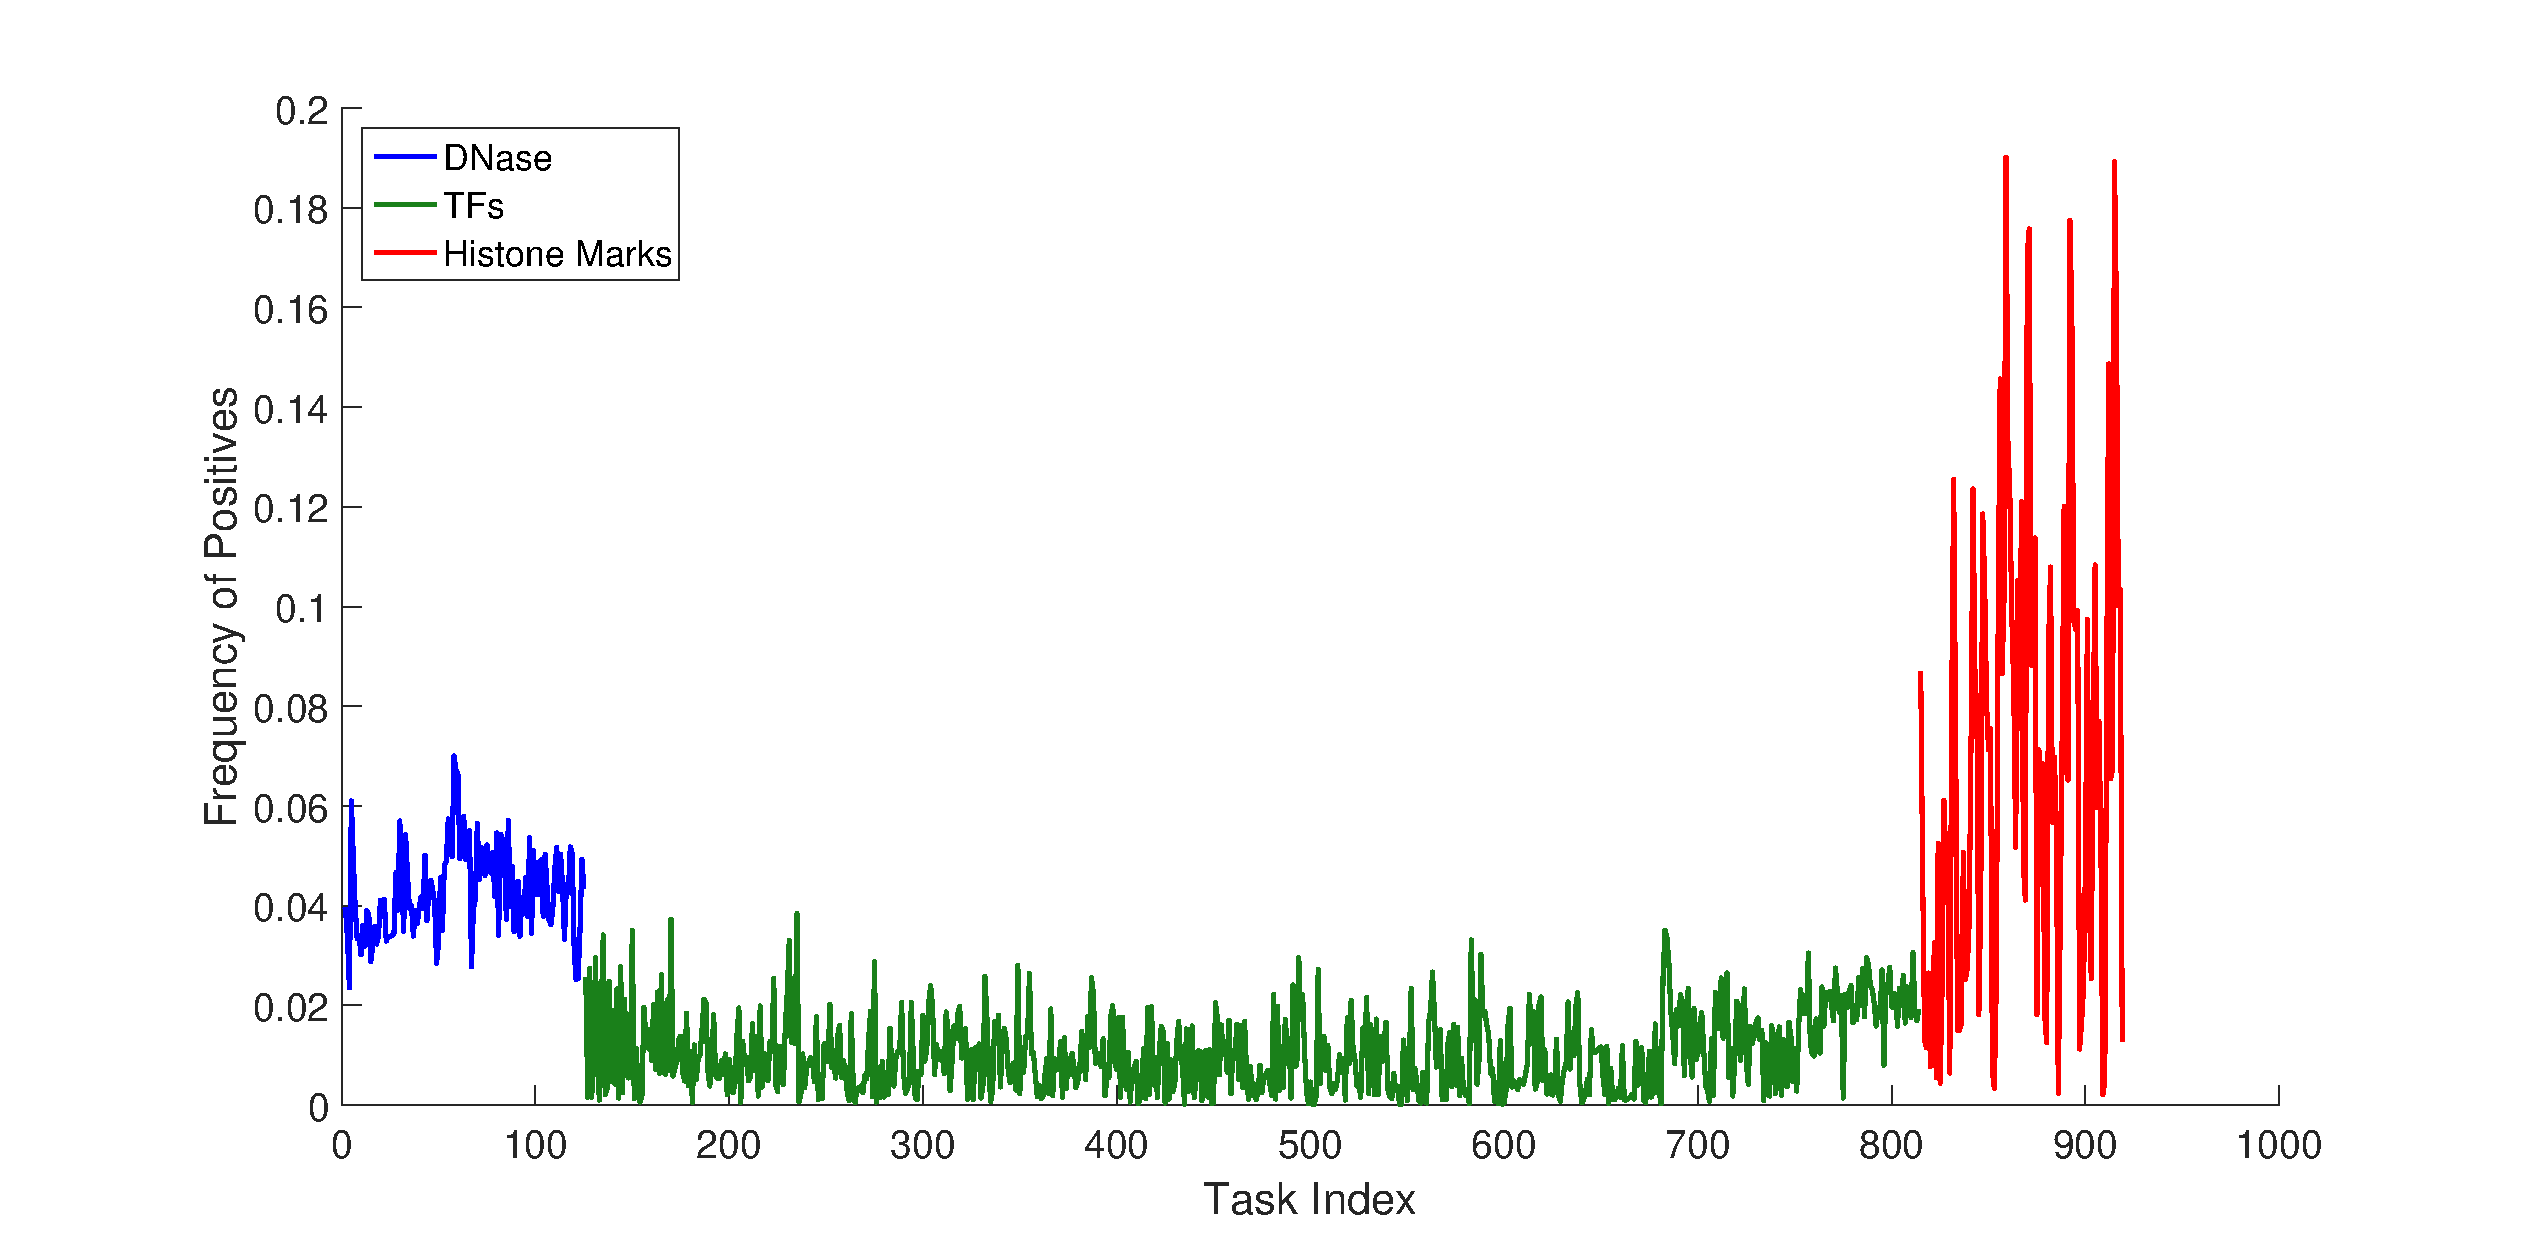
\includegraphics[width=1\textwidth]{figures/Frequency.eps}
\caption{Frequency of positive labels for each task.}
\label{fig:frequency}
\end{center}
\end{figure}

We experimented with the weighted negative-log-likelihood loss defined as
\begin{equation} \label{eq:weightedLoss}
-\sum_{i=1}^n \sum_{j=1}^m \alpha w_j I_{\{y_{i,j} = 0\}} \log(p_{i,j}) + (1- \alpha w_j) I_{\{y_{i,j} = 1\}}\log(1 - p_{i,j})
\end{equation}
where $n$ is the number of observations, $m$ is the number of tasks, and $I$ is the indicator function. To normalize the loss, for task $j$, the following weight was chosen:
\[
w_j = \frac{\mbox{Number of positive examples}}{n}
\]
We added some regularization to this weighting scheme by adding a parameter $\alpha$ that was set to $1.1$ after evaluating the performance of various choices on the validation set.

However, in our experiments, we were surprised to observe that adding the weights significantly hurts the results both in terms of ROC AUC and PR AUC.  While further tuning of the weighting scheme could result in improved performance, for the remainder of the results of this paper, we have employed the un-weighted loss function.

%\begin{enumerate}
%\item The weighting scheme suggested in (\ref{eq:weightedLoss}) puts massive weights on learning positive examples of rare TFs (Say of the order of 0.9999). If these rare positive cases are not predictable, we are essentially forcing our estimator to fit to noise. 
%\item Implementing the weighted loss in Keras is a complex task. The phenomenon that we are observing might be due to coding errors
%\end{enumerate}

\subsubsection{Regularization}
DeepSEA uses dropout as well as $L_1$ and $L_2$ regularization to avoid overfitting. We experimented with various choices of dropout, but we found that the model with no regularization performs the best in our case.

We trained each model for 10 epochs, while applying early stopping.  As seen in Figure \ref{fig:CNNlearningCurve} the learning tapers off fairly quickly. Although we did not explicitly regularize our model, we do not see signs of overfitting. It must be noted that the surprisingly low validation loss could be a result of the size of the validation set. The only form of regularization we have used is early stopping and limiting the training to 10 epochs. 

Figure \ref{fig:CNNlearningCurve} shows the learning curve for one such training. We have used the same validation set as in \cite{zhou2015predicting,quang2016danq}.


\begin{figure*}[h]
\begin{subfigure}[t]{0.47\textwidth}
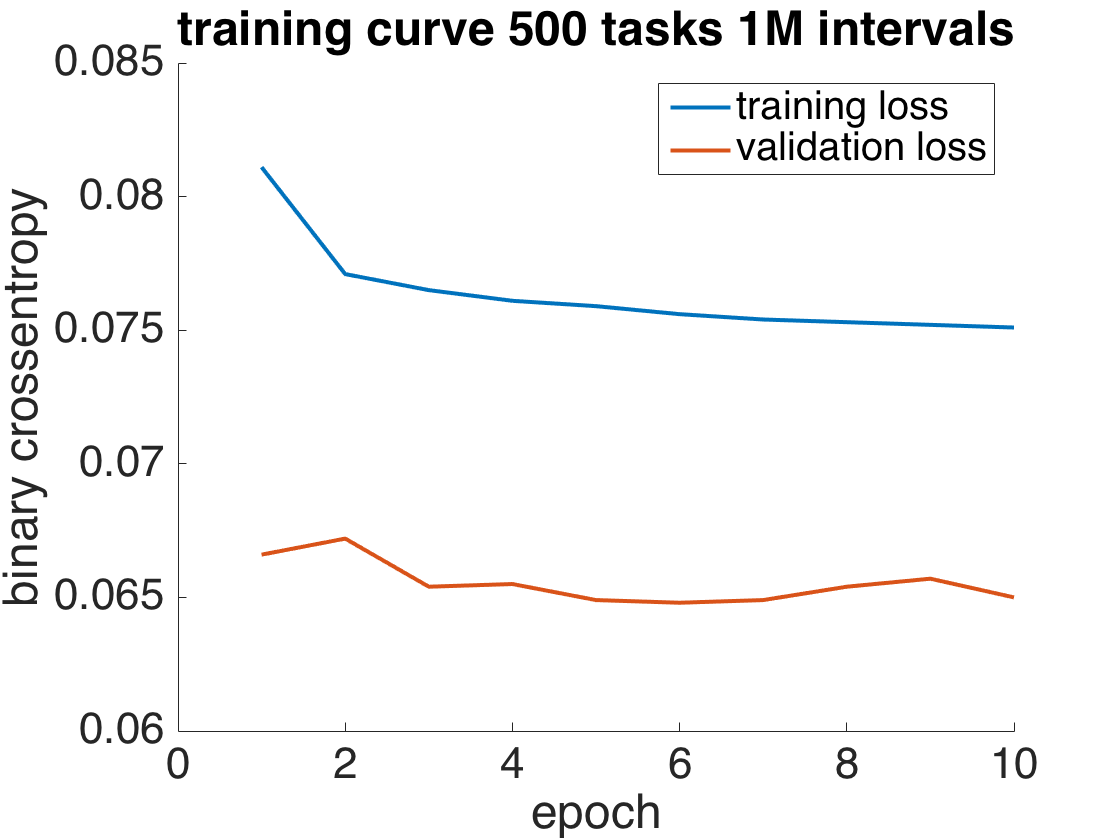
\includegraphics[width=\textwidth]{figures/learning_curve.png}
\caption{}
\end{subfigure}
\begin{subfigure}[t]{0.55\textwidth}
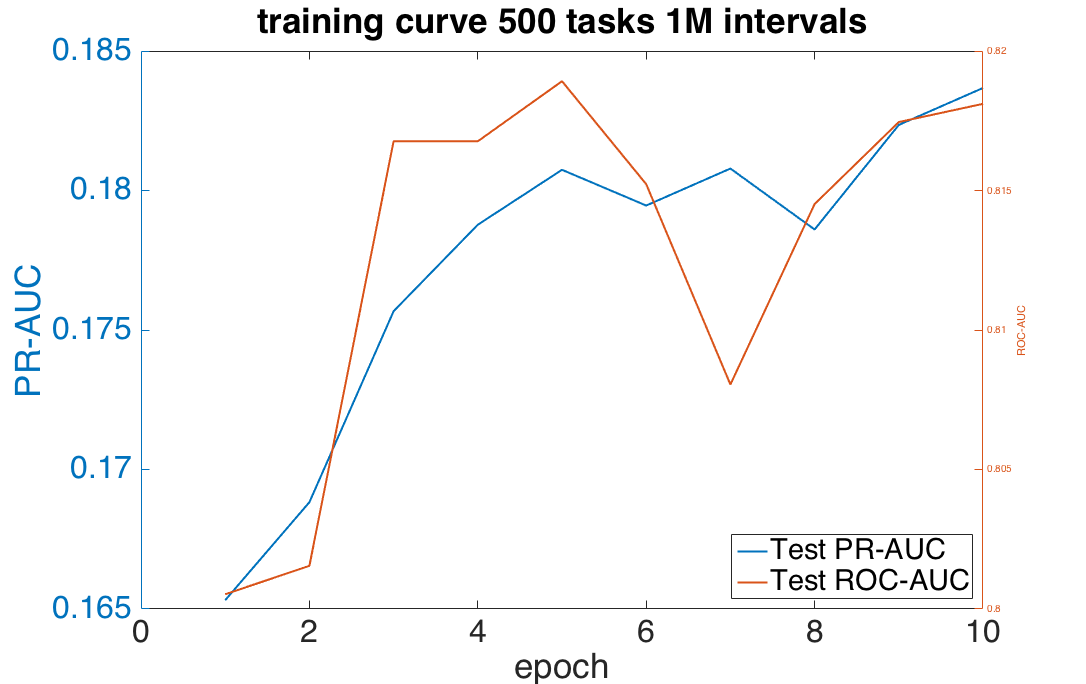
\includegraphics[width=\textwidth]{figures/AUCs.png}
\caption{}
\end{subfigure}
\caption{a) Training and validation loss for an example with 500 tasks and 1M regions. b) PR-AUC and ROC-AUC for the same example calculated on the test set}
\label{fig:CNNlearningCurve}
\end{figure*}

\subsection{Bidirectional Long Short-Term Memory Network}
Hyperparameters for our LSTM network were adapted from the choices made in the DanQ model \cite{quang2016danq}.  Namely, we made the LSTM bidirectional in order to incorporate sequence data flanking the current input on each side. Then, we applied a dropout regularization of 0.5 to the output of this bidirectional LSTM layer. Finally, we added a fully connected layer with ReLU input and sigmoid output activation functions to yield our multi-task output. This model was trained subject to an unweighted binary cross-entropy loss function using the RMSProp optimizer.  Due to computational limitations, 100K regions were used for training and testing.


% \subsubsection{CNN--Hyper-parameter search}

%An extension of the Long Short-Term Memory (LSTM) architecture, {\it sequence to sequence learning} [5], can be applied to model general sequence to sequence problems.  This method consists of two deep recurrent neural networks,  namely:

%\begin{itemize}
%\item an encoder network that processes the input and obtains a fixed-length representation
%\item a decoder network that generates the output of arbitrary length
%\end{itemize}

%This approach and related ones have been applied in [5], [6], and [7] and has achieved state-of-the-art results in machine translation and speech recognition tasks.  A graphical representation of this architecture can be seen in Figure \ref{fig:seq2seq}.

%\begin{figure}[!htbp]
%\centering
%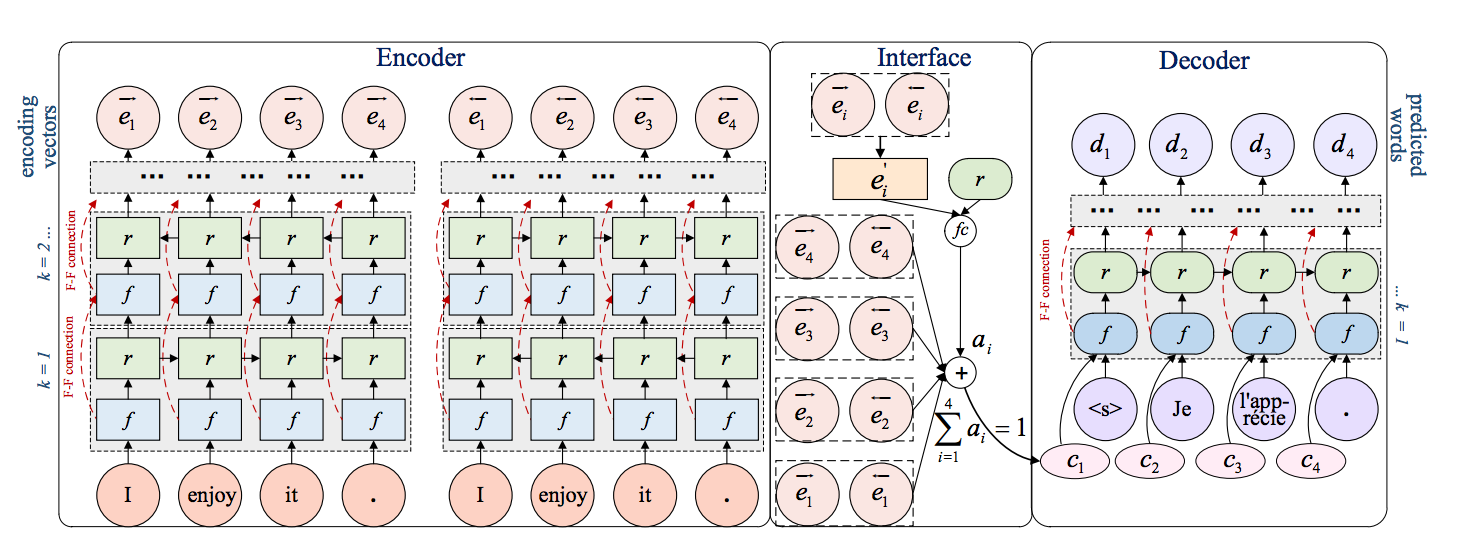
\includegraphics[width=\textwidth]{seq2seq_b.png}
%\caption{Graphical representation of sequence to sequence learning, using the example Deep-Att [8] architecture in a machine translation setting}
%\label{fig:seq2seq}
%\end{figure}

%Our objective is to compare the performance of two strategies.  First, we will use the sequence to sequence framework in the multi-task setting, to learn chromatin profiles directly from sequence (see Figure \ref{fig:approach1}).

%\begin{figure}[!htbp]
%\centering
%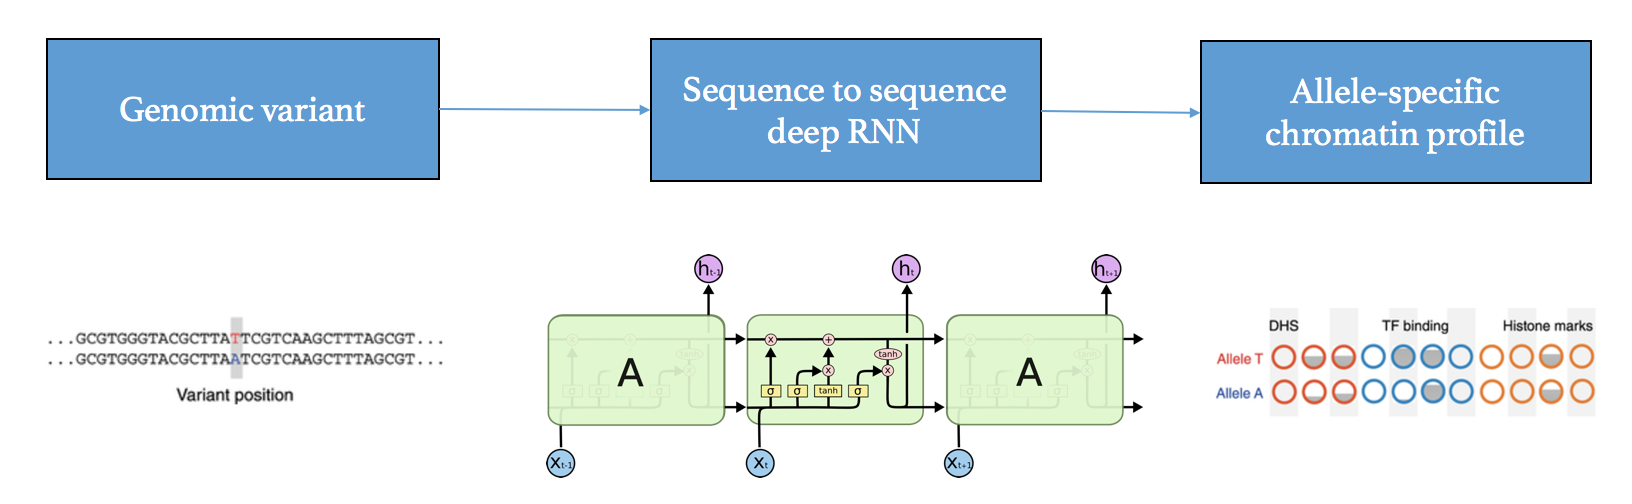
\includegraphics[width=\textwidth]{model1.png}
%\caption{Approach A: Directly predicting allele-specific chromatin profile from variant}
%\label{fig:approach1}
%\end{figure}

%Both DeepSEA and DanQ take advantage of CNNs as a motif discovery tool, due to their powerful modeling capacity for spatial features.  We anticipate that a fully recurrent architecture may not be as effective as discovering motifs.  As a second strategy, we will first convert a genomic variant to a matrix of ``motif scores.''  Subsequently, we will train a sequence-to-sequence RNN model on this motif-encoded sequence (see Figure \ref{fig:approach2}.)

%\begin{figure}[!htbp]
%\centering
%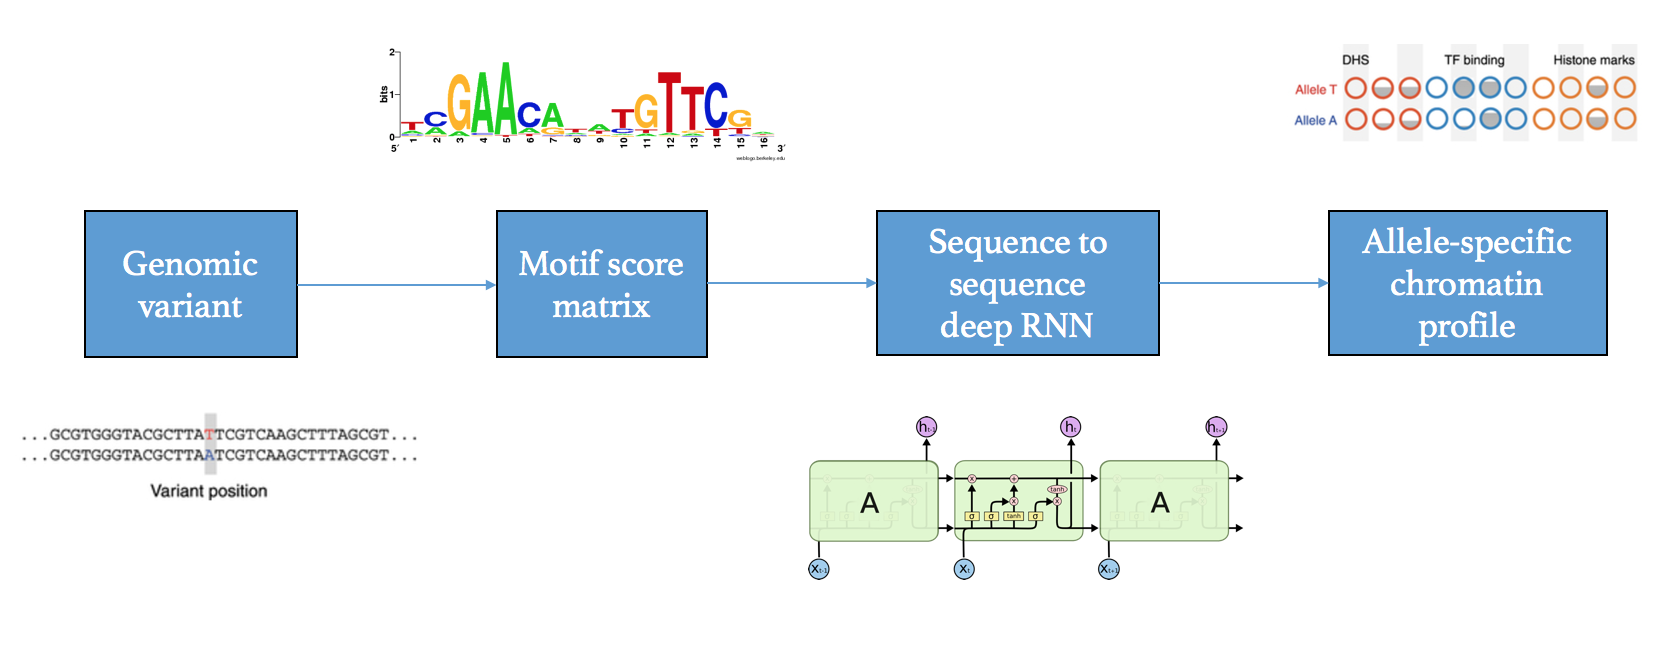
\includegraphics[width=\textwidth]{model2.png}
%\caption{Approach B: Computing a motif score matrix and then applying sequence to sequence learning}
%\label{fig:approach2}
%\end{figure}

%We aren't benchmarking against DeepSEA/DanQ I thought for multi-task approach. 
% In order to benchmark our approach against published algorithms, we will use chromatin profile data used by Zhou et al. [1].  We will use PR-AUC and ROC-AUC as performance metrics for chromatin profile prediction and we will benchmark our method against both the DeepSEA and DanQ models.
\section{Results}
We will split the results into two sections. In the first section we present our analysis of the performance characteristics of multitask learning.  Next, we will discuss our results training a Bidirectional LSTM directly on the input sequence.

\subsection{Multi-task learning performance analysis with CNN}

The results of runs from the model above are presented in the table \ref{tab:PR_Multitask}. In all cases, validation loss did not show signs of over-fitting. The table presents the PR-AUC on the training test for the model at the 10th epoch. The training regions are constant across rows and the larger multi-task settings include all the tasks from smaller settings.

From these results, we see that the performance increases as the number of tasks considered increase. Further analysis could investigate 1) whether this increase tapers off after a certain number of tasks and 2) how much this increase changes with the amount of data available. 

\begin{table}[h]
\begin{center}
\begin{tabular}{ |c|c|c|c| } 
 \hline
  & 100 tasks & 300 tasks & 500 tasks \\
 \hline
 750k regions & -- & 0.175 & -- \\ 
 \hline
 1Mk regions & 0.168 & 0.191 & 0.184 \\ 
 \hline
\end{tabular}
\vspace{6pt}
\caption{Precision-recall AUC on the testing set for various combinations of training sizes and tasks sizes}
\label{tab:PR_Multitask}
\end{center}
\end{table}

Furthermore, as we discussed earlier, the extent of imbalance in these tasks is different. The presence of different clusters within the tasks can be further observed after dimensionality reduction. From Figure \ref{fig:pca} we can clearly detect two separate clusters for TF's and one cluster for DNase. Histone markers do not seem to cluster very well.

We ran an experiment training our network on 100 DNase tasks. The PR-AUC results can be seen in Table~\ref{tab:PR_DNase}. We have compared the average PR-AUC from the DNase-only training to 1) the average results from 100 random tasks training and 2) the average only on the shared subset (size = 11) between our random task training and our DNase-only tasks training. Note that in all cases the training task size is 100. The results can be seen in Table \ref{tab:PR_DNase}. This provides preliminary evidence that training on similar tasks is beneficial to performance.

\begin{table}[h]
\begin{center}
\begin{tabular}{ |c|c|c|c| } 
 \hline
   & 100 DNAse only & 100 random tasks & 100 rnd. tasks Eval. on DNase only \\
 \hline
 1M regions & {\bf 0.258} & 0.168 & 0.222\\
 \hline
\end{tabular}
\vspace{6pt}
\caption{Average PR-AUC for different multi-task learning formulations with 100 tasks and 1M regions.}
\label{tab:PR_DNase}
\end{center}
\end{table}

\begin{figure}
\hspace{-40pt}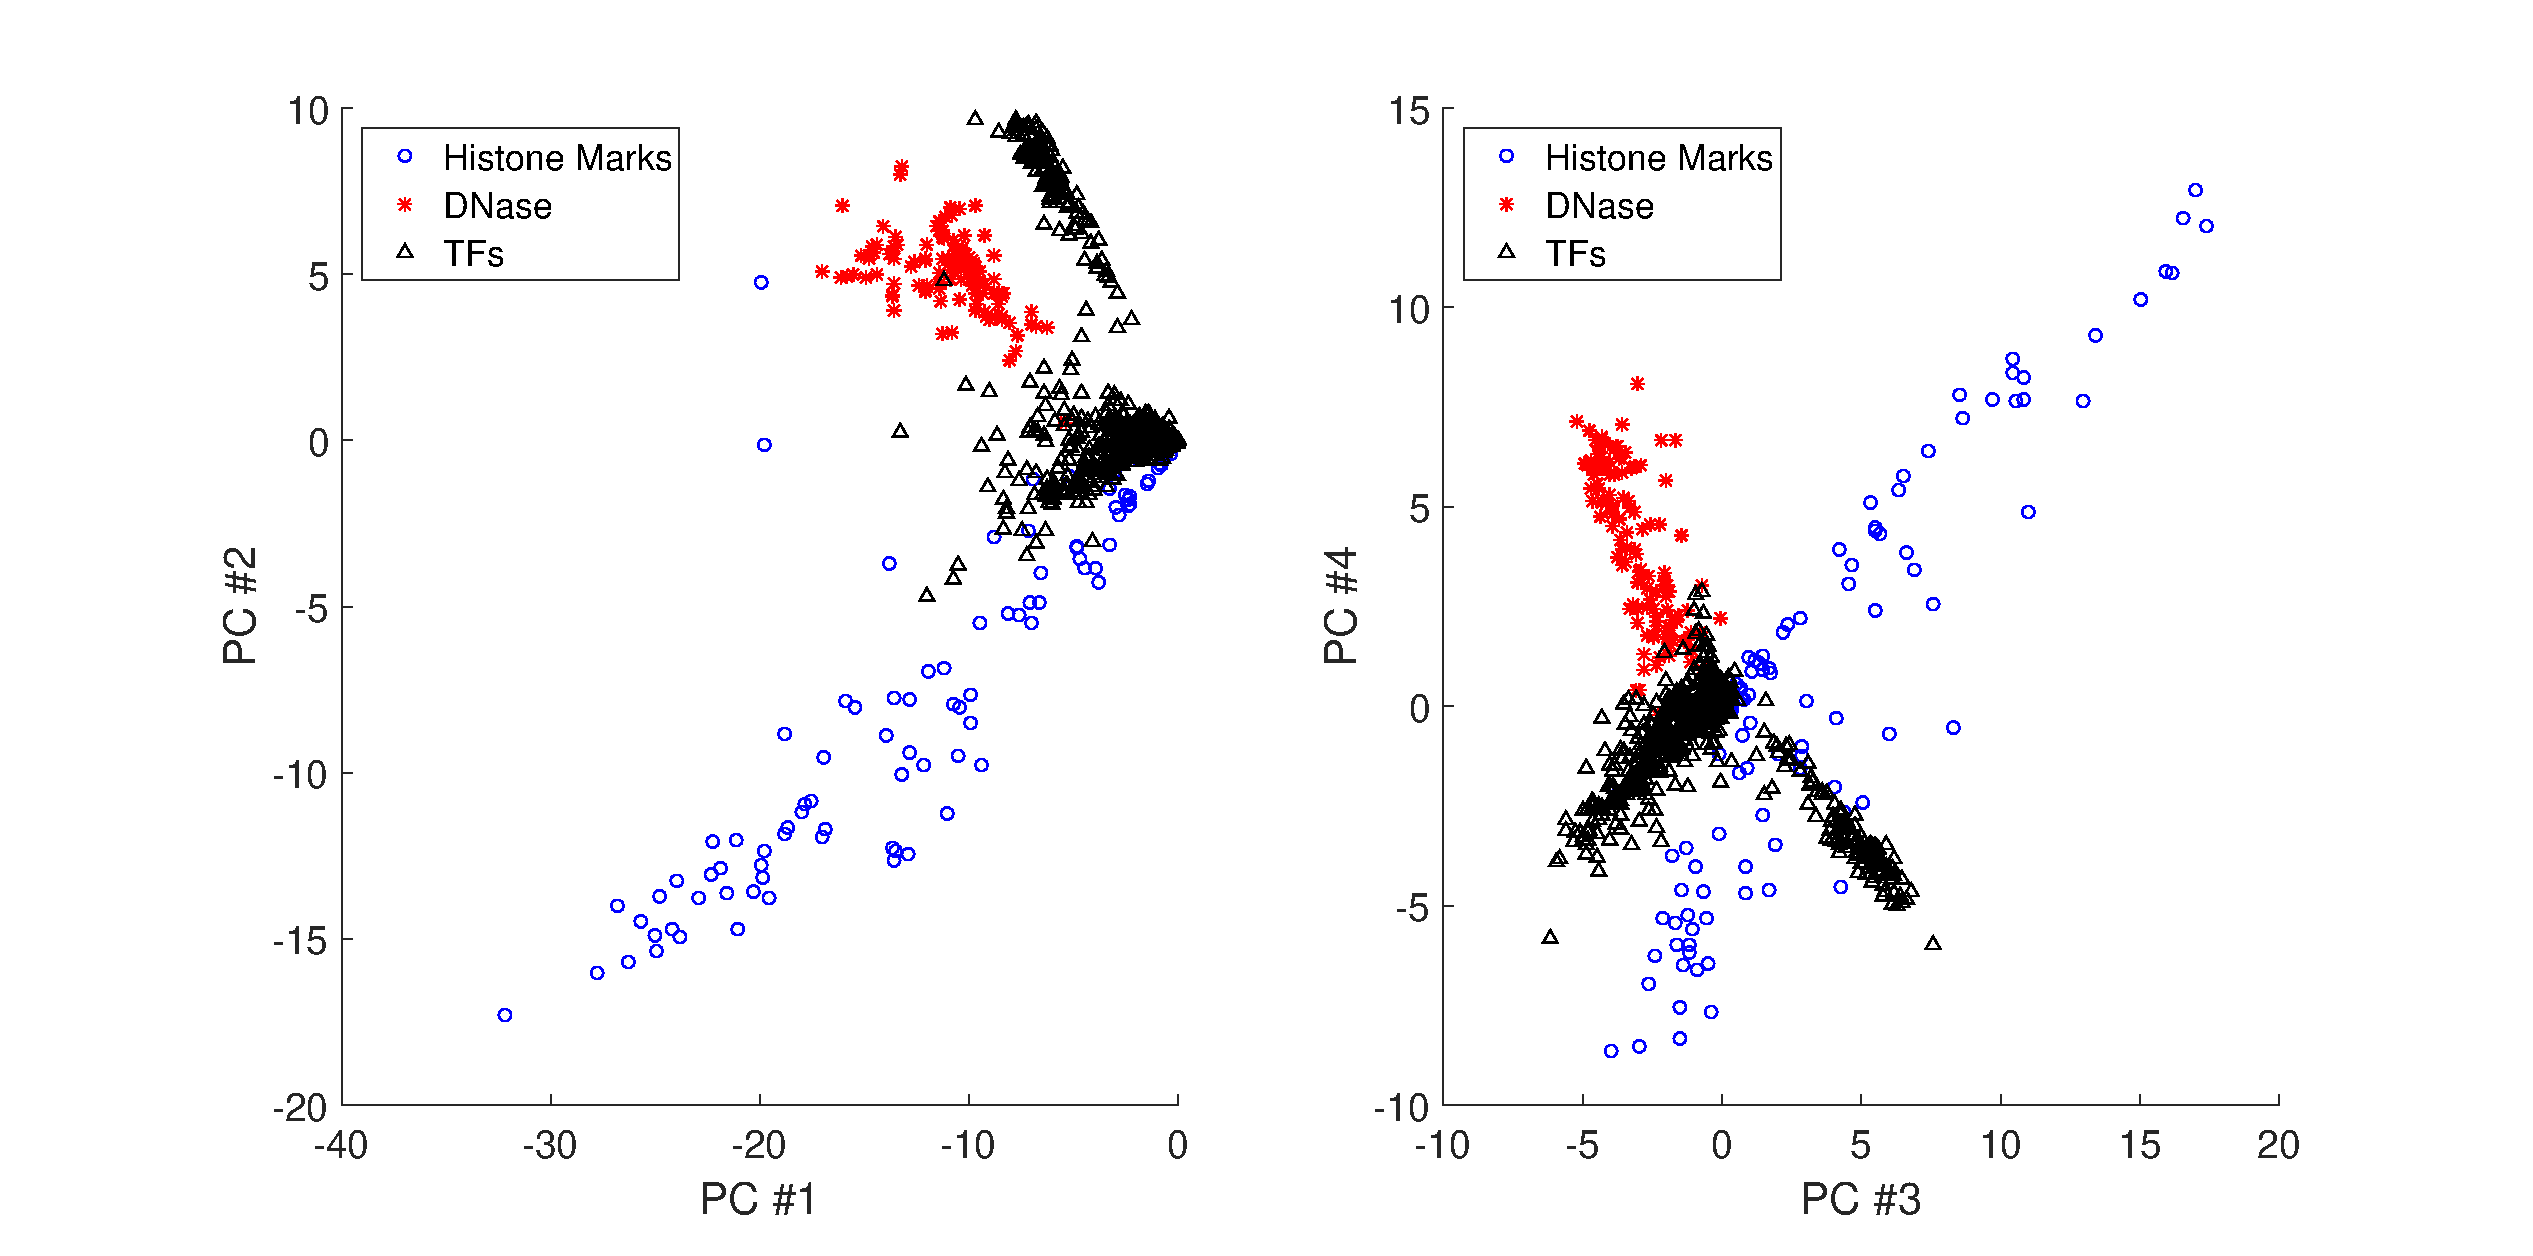
\includegraphics[width=1.2\textwidth]{figures/PCS.eps}
\caption{PCA plot of binding location of each task calculated from the first 10,000 regions. DNASE forms a clear cluster, TFs form two separated clusters and Histone markers do not cluster well.}
\label{fig:pca}
\end{figure}

\subsection{Bidirectional LSTM Network}
To analyze the model of our bidirectional-LSTM network, we computed 919 receiver operating characteristic and precision-recall curves.  As noted in \cite{quang2016danq}, PR curves in particular often provide a more robust measure of performance when training data exhibits class-imbalance.  

Below we report the distribution of the area under each ROC curve (Figure \ref{fig:rocauc}), as well as each PR curve (Figure \ref{fig:aucpr}).  The AUC PR values were compared to task-specific logistic regression baselines mentioned in the DeepSEA paper \cite{zhou2016deep}.  Notably, the bidirectional LSTM model outperforms this baseline even when trained on a small subset of the available training data.

\begin{figure}[h]
\centering 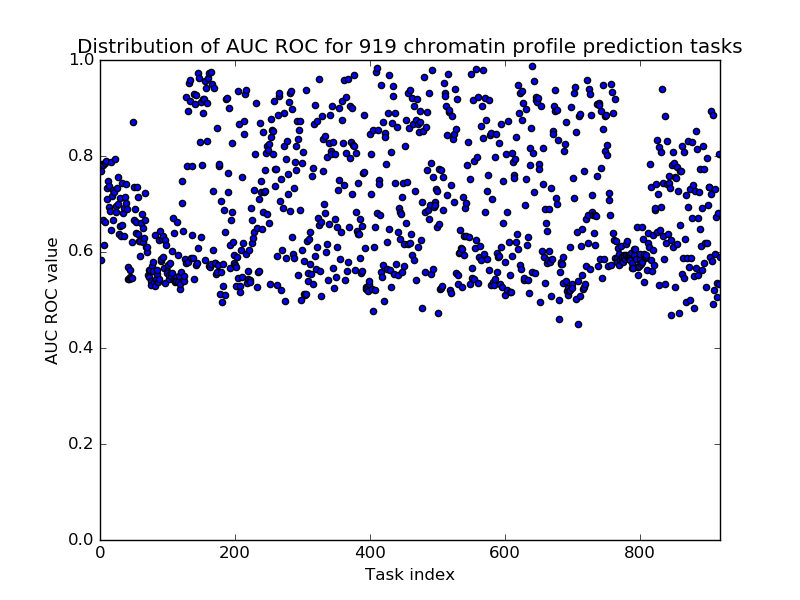
\includegraphics[width=.7\textwidth]{figures/roc_aucs.png}
\caption{Distribution of AUC ROC for 919 chromatin profile prediction tasks}
\label{fig:rocauc}
\end{figure}

\begin{figure}[h]
\centering 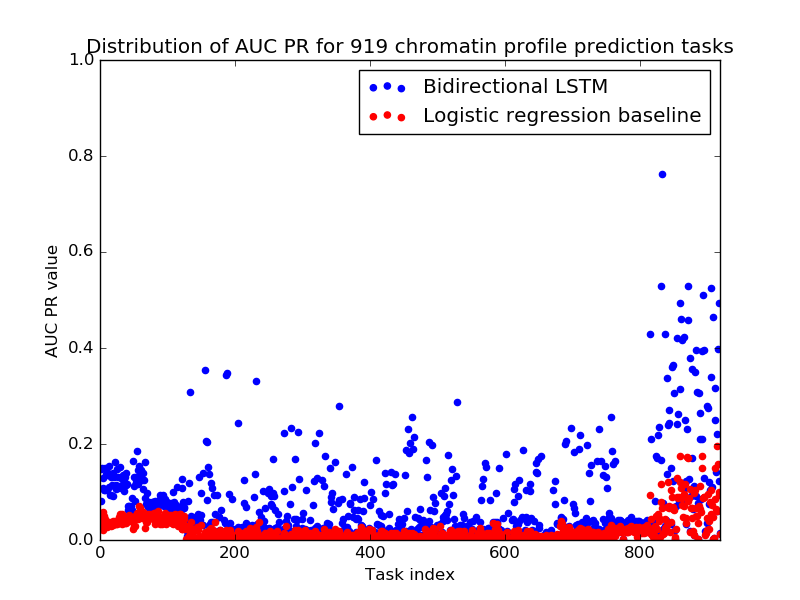
\includegraphics[width=.7\textwidth]{figures/avg_precs2.png}
\caption{Distribution of AUC PR for 919 chromatin profile prediction tasks}
\label{fig:aucpr}
\end{figure}

We have also produced example ROC curves for particular tasks.  In the figures below, we present the model's performance on task 639, predicting NELFe transcription factor binding on the K562 cell type, as well as task 493, predicting ZNF263 transcription factor binding on the HEK293-T-REx cell type.  Task 639 was the best performing in terms of AUC ROC, while task 493 was a randomly selected task, closer to the average AUC ROC value.

\begin{figure}[h]
\centering 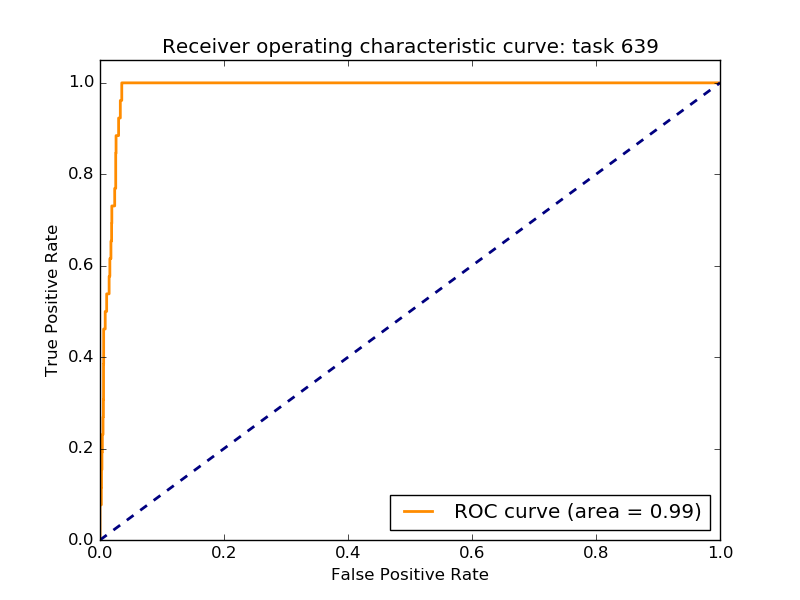
\includegraphics[width=.7\textwidth]{figures/roc_example639.png}
\caption{ROC curve: task 639, predicting NELFe transcription factor binding on the K562 cell type}
\label{fig:t1}
\end{figure}

\begin{figure}[h]
\centering 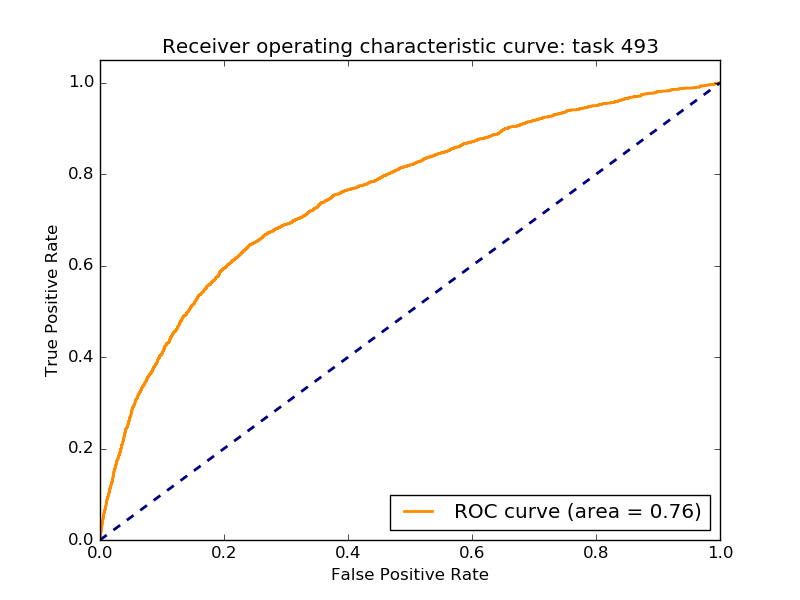
\includegraphics[width=.7\textwidth]{figures/roc_example493.png}
\caption{ROC curve: task 493, predicting ZNF263 transcription factor binding on the HEK293-T-REx cell type}
\label{fig:t2}
\end{figure}

Similarly, we present example PR curves for individual tasks.  In the figures below, we display the model's performance on task 832, predicting H3K4me3 methylation on the H1-hESC cell type, as well as task 848, predicting H3K4me3 methylation from the K562 cell type.  Task 832 was the best performing task in terms of AUC PR, while task 848 was a randomly selected task, more representative of average performance.

\begin{figure}[h]
\centering 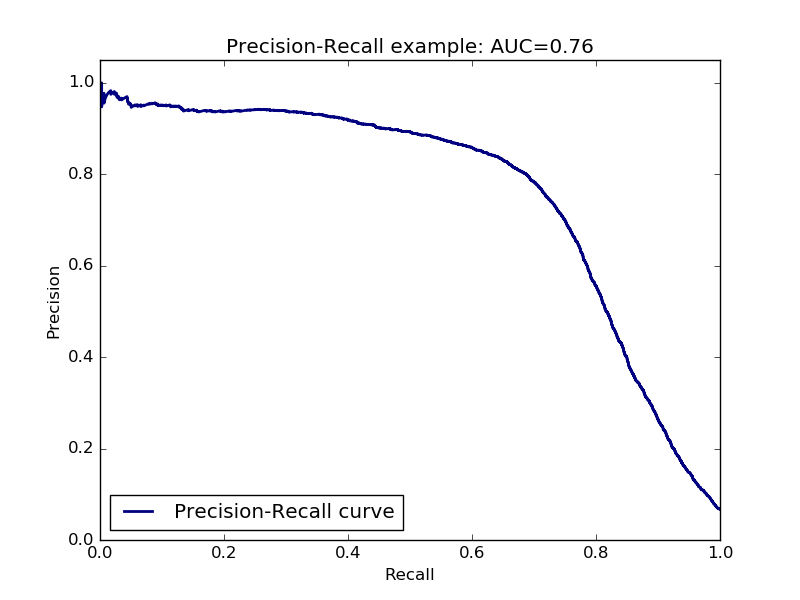
\includegraphics[width=.7\textwidth]{figures/pr_example832.png} 
\caption{PR curve: task 832, predicting H3K4me3 methylation on the H1-hESC cell type}
\label{fig:t3}
\end{figure}

\begin{figure}[h]
\centering 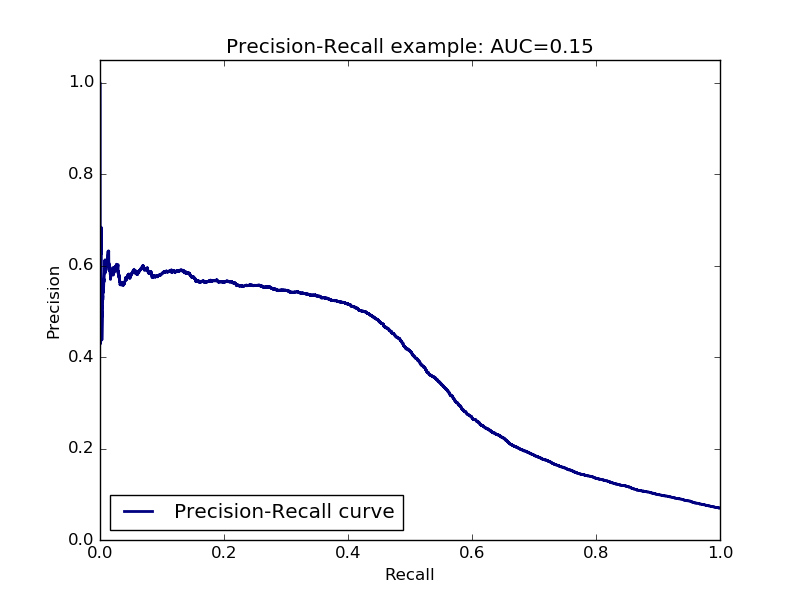
\includegraphics[width=.7\textwidth]{figures/pr_example848.png}
\caption{PR curve: task 848, predicting H3K4me3 methylation from the K562 cell type}
\label{fig:t4}
\end{figure}


\section{Conclusion and Future Work}
We have demonstrated a proof-of-concept for applying fully recurrent neural networks to the problem of multi-tasked chromatin profiling prediction. Namely, our promising results for the bidirectional LSTM network suggest that an intermediate convolutional neural network layer might not be necessary.  By using extensions of this fully recurrent model, we can model input sequences of arbitrary length and model long range interactions.

\par
Furthermore, in this work we have also analyzed the performance characteristics of multi-task learning. We see that multi-task learning and increasing the number of tasks does indeed improve the results.  Furthermore, we studied the distribution of clusters that may be well suited for mutual learning. Specifically, we show that DNase, and TF tasks seem to form well defined clusters and we produce hints that learning based on these boundaries may be particularly beneficial.

In the future, we would like to further investigate the multi-task learning curve. Our results hint that after 300 tasks the benefits may be small however, more extensive experimentation is needed to account for the stochasticity  of learning. Additionally, we would like to experiment with other sets of tasks that may be particularly well-suited for multi-task learning (e.g. tasks within a cell-type). We also need to further study our current hypothesis that multi-task learning segmented by the type of task is a beneficial formulation. More hyper-parameter search and repetitions would help quantify the extent/existence of a signal. 

%Furthermore, we see that at 750k regions additional data seem to have substantial effect on improving the results (this may explain some of the discrepancy between the PR-values in this work and those obtained by DeepSEA \cite{zhou2015predicting}).

\par
For our recurrent model, we would like to refine our performance by training on the entire data set and performing a more extensive hyper-parameter search. Additionally, it might prove useful to experiment more with our architecture by training a deeper model. For these experiments we have relied on data provided by previous works which contain a 1000bp context size. For future work, the efficacy of LSTM's in learning long range interactions can be examined by increasing this window size.

\par
We would also like to extend our fully recurrent model to other variants of RNNs. Namely, we would like to investigate the suitability for Clockwork RNNs on the present problem. Clockwork RNN (CWRNN), a new variant of RNN architecture \cite{koutnik2014clockwork} have recently been introduced by Schmidhuber et al.  CWRNN utilizes clocked module activation and divides hidden layers into modules with distinctive temporal granularity, and it embodies both short-term and long-term dependencies by specializing units that operate on a defined timescale. This reduces the number of overall RNN parameters, and the empirical results shows significant improvement and acceleration across several language modeling training tasks.  In particular, they outperform standard RNNs and LSTMs on sequence generation form audio waveform, and spoken word classification experiments. We think this framework might be potentially suited for the task of chromatin profile prediction in which long-range interactions are present. While CWRNN has received some success in analyzing language waveform data, which have implicit periodic structure, its performance on gene sequential data has not been explored. More research needs to be conducted to study the optimal time scaling mechanisms as well its applications in the chromatin profile prediction tasks with genome data.
\bibliography{Bibliography}

\end{document}